\documentclass[scheme=plain,12pt]{ctexart}

\usepackage{graphicx}
\usepackage{amsthm}
\usepackage{amsmath}
\usepackage{amssymb}
\usepackage[hmargin=1.1in,vmargin=1in]{geometry}
\usepackage{indentfirst}
\usepackage[defaultmono]{droidsansmono}
\usepackage[xetex,colorlinks=true]{hyperref}

\fontsize{14pt}{1.0}

\newlength{\blanklength}
\setlength{\blanklength}{40ex}

\providecommand{\thetitle}{Homework of Chapter 02}
\providecommand{\theauthor}{Sparky\_14145}
\providecommand{\thestudentID}{71XXXXXX}
\providecommand{\theemail}{Sparky\_14145@outlook.com}
\providecommand{\theinstitution}{College of Software Engineering}

\input{personal_info/info.tex}

\providecommand{\blankToFill}[1]{
    \parbox[t][3ex]{\blanklength}{
        \makebox[\blanklength]{#1}\\[0pt]
        \rule[2ex]{\blanklength}{0.1ex}
    }
}

\providecommand{\makecover}{\begin{titlepage}
    \noindent
    {Course Homework} \\[2pt]
    {\large \bfseries Southeast University}

    \vspace*{70pt}
    \begin{center}
        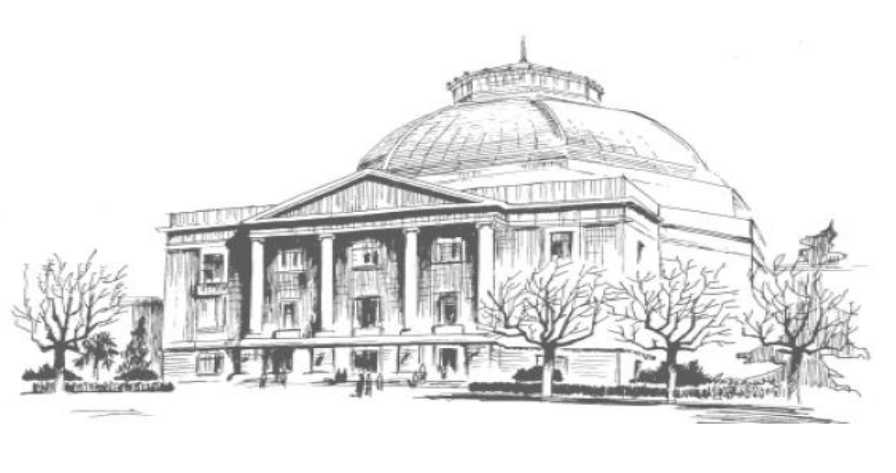
\includegraphics[width=0.9\textwidth]{pics/cover.png} \\[2pt]
        \textsc{\Huge Principles of Compilers}\\[10pt]
        \begin{tabular}[c]{rc}
            Title       & \blankToFill{\thetitle} \\
            Date        & \blankToFill{\today} \\
            Author      & \blankToFill{\theauthor\footnotemark} \\
            Student ID  & \blankToFill{\thestudentID} \\
            Institution & \blankToFill{\theinstitution}
        \end{tabular}
        \rmfamily
    \end{center}
    \footnotetext{\theemail}
\end{titlepage}}

\begin{document}
    \makecover

    \section{T2.2.1}

    Considet the given context-free grammar:

    \[
        S \to S\;S\;\mathtt{+}\;|\;S\;S\;\mathtt{*}\;|\;\mathtt{a}
    \]

    \begin{enumerate}
        \item Show how to generate the string \verb|aa+a*|;
        \item Construct a parse tree to the string;
        \item What's the language generated by the grammar? Prove it.
    \end{enumerate}

    \paragraph*{Solution: }
    \begin{enumerate}
        \item \begin{enumerate}
                \item First we transform $S$ to $S\;S\;\mathtt{*}$;
                \item Then we transform the first $S$ to $S\;S\;+$, and the second one to \verb|a|, resulting $S\;S\;\mathtt{+a*}$;
                \item Finally transform the leading $S$s to \verb|a|, resulting \verb|aa+a*|. That's it.
              \end{enumerate}
        \item See figure \ref{fig:t1-1}.
              \begin{figure}[h]
                \centering
                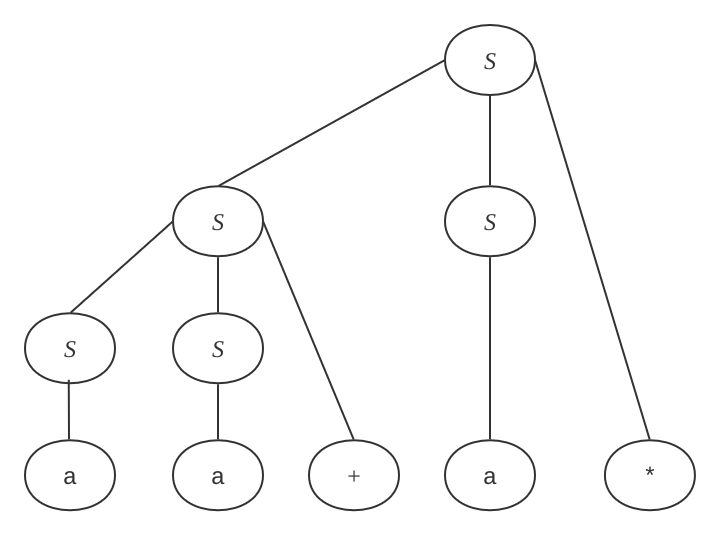
\includegraphics[width=0.5\textwidth]{pics/t1-1.png}
                \caption{Parse Tree of the String \texttt{aa+a*}}
                \label{fig:t1-1}
              \end{figure}
        \item A language of postfix notations whose operators $op \in \{+, *\}$, and the only operand is $\mathbf{a}$.
        \begin{proof}
            We know that $\mathbf{a}$ is a vaild postfix notation, which can be generated by $S \to \mathbf{a}$.

            Then for any vaild postfix notation $S_1, S_2$, both $+\,S_1\,S_2$ and $*\,S_1\,S_2$ are vaild postfix notations too.
            
            So the given grammar generates a language notations of postfix notations.
        \end{proof}
    \end{enumerate}

    \newpage
    \section{T 2.2.2}

    What language is generated by the following grammars? In each justify your answer.

    \begin{enumerate}
        \item $S \to 0\,S\,1\;|\;0\,1$
        \item $S \to +\,S\,S\;|\;-\,S\,S\;|\;\mathbf{a}$
        \item $S \to S\,(\,S\,)\,S\;|\;\varepsilon$
        \item $S \to \mathbf{a}\,S\,\mathbf{b}\,S\;|\;\mathbf{b}\,S\,\mathbf{a}\,S\;|\;\varepsilon$
        \item $S \to \mathbf{a}\;|\;S\,+\,S\;|\;S\,S\;|\;S\,*\;|\;(\,S\,)$
    \end{enumerate}

    \paragraph*{Solutions:}
    \begin{enumerate}
        \item $L = \{0^n1^n | n \geq 1\}$
        \begin{proof}
            First we have $S \to 0\,1$, so $0^11^1 \in L$.

            Then for any $n \geq 1$, assume that $S = 0^n1^n \in L$, then $S' = 0S1 = 0^{n+1}1^{n+1} \in L$.

            So for any string $S$ generated by the syntax, $S \in L$.
        \end{proof}
        \item A language of prefix notations whose operands are $+$ and $-$, and the only operand is $\mathbf{a}$.
        \item $L = \left\{\omega\in\Bigl(\,(\,\Big|\,)\,\Bigr)^* \Big| \text{All brackets in }\omega\text{ matches.}\right\}$
        \begin{proof}
            If $\omega = \varepsilon$, which is generated by $S \to \varepsilon$, then obviously all brackets in $\omega$ matches (since there is no bracket in $\omega$).

            If $\omega_1, \omega_2, \omega_3 \in L$, we know that brackets in $(\,\omega_2\,)$ matches, then all brackets in $\omega_1(\omega_2)\omega_3$, generated by $S \to S\,(S)\,S$, matches.

            Assume $s$ is is a string from $L$. If $s = \varepsilon$, then $s$ matches $S \to \varepsilon$.

            Otherwise take the leading bracket $B_1$ (which must be a left bracket), and its matching bracket $B_2$, then the string $s$ can be expressed as
            \[\varepsilon B_1 \omega_1 B_2 \omega_2\]
            Where $\omega_1, \omega_2 \in L$, matching $S \to S\,(\,S\,)\,S$.

            So the given grammar generates language $L$.
        \end{proof}
        \item $L = \{(\mathbf{a}\,|\,\mathbf{b})^* | \text{Number of \textbf{b} is equal to of \textbf{a}.}\}$
        \begin{proof}
            To show that any string $s$ generated by the grammar belongs to language $L$:
            \begin{enumerate}
                \item If $s = \varepsilon$, generated by $S \to \varepsilon$, then obviously number of $\mathbf{b}$ is equal to of $\mathbf{a}$ (= 0).
                \item Then assume that $s_1, s_2 \in L$. By applying $S \to \mathbf{a}\,S\,\mathbf{b}\,S\;|\;\mathbf{b}\,S\,\mathrm{a}\,S$, we get $s_1' = \mathrm{a}s_1\mathrm{b}s_2$, or $s_2' = \mathrm{b}s_1\mathrm{a}s_2$, whose number of $\mathbf{b}$ is also equals to of $\mathbf{a}$.
                \item So any string generated by the grammar belongs to language $L$.
            \end{enumerate}
            To show that any string $s \in L$ can be generated by the grammar:
            \begin{enumerate}
                \item If $s = \varepsilon$, matching $S \to \varepsilon$, then obviously it can be generated.
                \item Otherwise if $s$ begins with $\mathbf{a}$, then find its matching $\mathbf{b}$ (we say an $\mathbf{a}$ matches a $\mathbf{b}$, iff the substring between the two symbols belongs to $L$, and the length of the substring is minimal). The symbols split $s$ into $\mathrm{a}s_1\mathrm{b}s_2$, where $s_1, s_2 \in L$ obviously, matching $S \to \mathbf{a}\,S\,\mathbf{b}\,S$.
                \item If $s$ begins with $\mathbf{b}$, we can split it as it begins with $\mathbf{a}$, and finding it matches $S \to \mathbf{b}\,S\,\mathbf{a}\,S$.
            \end{enumerate}
            So the language $L$ can be generated by the given grammar.
        \end{proof}
        \item A language of infix notations.
    \end{enumerate}

    \newpage
    \section{T 2.2.4}

    Construct unambiguous context-free grammars for each of the following languages. In each case show that your grammar is correct.

    \begin{enumerate}
        \item Arithmetic expressions in postfix notation.
        \item Left-associative lists of identifiers separated by commas.
        \item Right-associative lists of identifiers separated by commas.
        \item Arithmetic expressions of integers and identifiers with the four binary operators $+, -, \times, \div$.
        \item Add unary plus and minus to the arithmetic operators of (4).
    \end{enumerate}

    \paragraph*{Solutions:}

    Let's define some common non-terminals first:

    \begin{enumerate}
        \item $digit \to [0-9]$;
        \item $pnumber \to 0\;|\;[1-9]digit^*$;
        \item $number \to (+|-)?pnumber$;
        \item $char \to \mathbf{a}-\mathbf{z}|\mathbf{A}-\mathbf{Z}$;
        \item $identifier \to (\_|char)(\_|char|digit)^*$.
    \end{enumerate}

    Then the solutions:

    \begin{enumerate}
        \item \begin{align*}
            expression  &\to [+-\times\div]\;expression\;expression \\
            expression  &\to number
        \end{align*}
        \item \begin{align*}
            list        &\to list,\;identifier \\
            list        &\to identifier
        \end{align*}
        \item \begin{align*}
            list        &\to identifier,\;list \\
            list        &\to identifier
        \end{align*}
        \item \begin{align*}
            expression  &\to expression\;[+-]\;item \\
            expression  &\to item \\
            item        &\to item\;[\times\div]\;factor \\
            item        &\to factor \\
            factor      &\to  (\;expression\;) \\
            factor      &\to pnumber\;|\;identifier
        \end{align*}
        \item \begin{align*}
            expression  &\to expression\;[+-]\;item \\
            expression  &\to item \\
            item        &\to item\;[\times\div]\;sfactor \\
            item        &\to sfactor \\
            sfactor     &\to [+-]\;factor \\
            factor      &\to  (\;expression\;) \\
            factor      &\to pnumber\;|\;identifier
        \end{align*}
    \end{enumerate}
\end{document}